\documentclass[12pt,letterpaper]{scrartcl}
%\documentclass[12pt,letterpaper]{article}
\usepackage[margin=1in]{geometry}
\usepackage[superscript,biblabel]{cite}
\usepackage{url,graphicx,xcolor,enumitem}

%opening
\title{A Tutorial on PCB Design}
\subtitle{--- using KiCad}
\author{Xiaoguang ``Leo'' Liu \\University of California Davis \\ lxgliu@ucdavis.edu}
\date{Aug.~9th, 2015}

\begin{document}

\maketitle

\tableofcontents

\newpage
\section{PCB Basics}

\subsection{Example 2: A 2.4\,GHz low noise amplifier (LNA)}

\newpage
\section{KiCad}
In the early days, PCBs are designed and laid out literally by hand. See Fig.~\ref{fig:hand-pcb} for an example board from that era. As technologies developed, it become more common to do the job with the help of a computer. Today, there are numerous software tools for PCB design. On the high end, industry-grade packages, such as Cadence Allegro~\footnote{UC Davis students have access to the full suite of Allegro PCB design tools through a donation from Cadence.}, Mentor Graphics Xpedition, and Altium Designer, offer extensive features and capabilities with a high price tag and often a very steep learning curve. On the lower end, popular choices include CadSoft EAGLE, ExpressPCB, and DesignSpark, all of which offer a reasonable set of features at an affordable price. 

\begin{figure}[ht]
\centering
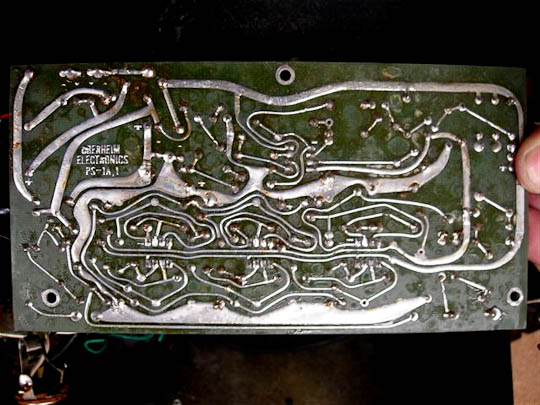
\includegraphics[width=2.5in]{hand-pcb.jpg}
\caption{A vintage PCB laid out by hand~\cite{hand-pcb}.}
\label{fig:hand-pcb}
\end{figure}

In recent years, KiCad has emerged as a popular open-source software package for designing and laying out PCBs~\cite{kicad}. KiCad is available on all three major personal computer operating systems, Windows, Linux, and Mac OS. 
Compared with the above mentioned software packages, KiCad is completely free of charge or any other limitation. Although KiCad is not as sophisticated as industry-level tools, it is capable of dealing with fairly complicated designs, and the active developer community is working hard to improve its capabilities. In fact, as of this writing, KiCad has not had an official stable release for the last two years because of the constant development progress being made. In this tutorial, we will using a recent build \#6055, dated Aug.~8th, 2015.

Fig.~\ref{fig:kicad-main} shows the main window of KiCad. The main window serves as a project management panel where you can launch the individual PCB tools. 

\begin{figure}
\centering
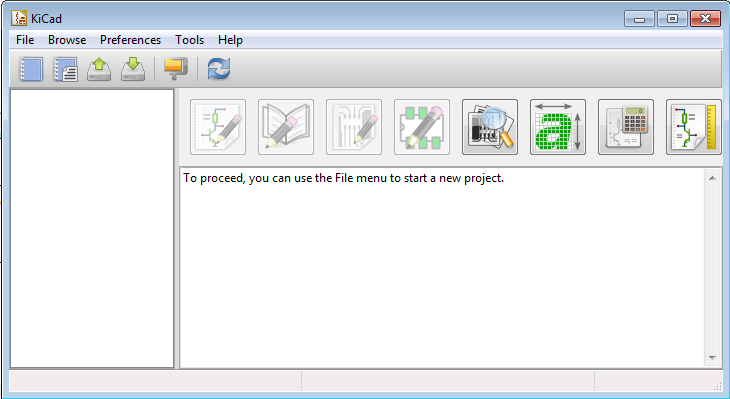
\includegraphics[width=5in]{kicad-main.png}
\caption{The main window of KiCad.}
\label{fig:kicad-main}
\end{figure}

\begin{table}
\caption{Individual tools within KiCad.}
\begin{tabular}{|c|c|}
\hline 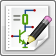
\includegraphics[width=0.5in]{eeschema-icon}  &   Eeschema: schematic editor/capture tool\\ 
\hline 
\includegraphics[width=0.5in]{sche-lib-icon} &  Schematic symbol editor\\ 
\hline 
\includegraphics[width=0.5in]{pcbnew-icon} &  Pcbnew: PCB layout tool\\ 
\hline 
\includegraphics[width=0.5in]{footprint-lib-icon} &  Component footprint editor\\ 
\hline 
\includegraphics[width=0.5in]{gerbview-icon} &  Gerbview: Gerber file viewer\\ 
\hline 
\includegraphics[width=0.5in]{bitmap2component-icon} &  Bitmap2Component: A tool for creating component symbol from a picture\\ 
\hline 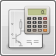
\includegraphics[width=0.5in]{calculator-icon} &  A calculator for common PCB design related calculations \\ 
\hline 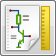
\includegraphics[width=0.5in]{pi-editor-icon} &  Schematic sheet layout editor\\ 
\hline 
\end{tabular} 
\end{table}

\section{Example 1: Arduino dice}
In the first example we will make a small eletronic dice consisting of a ATmega328P microcontroller---the heart of the popular Arduino UNO platform, a switch, a 7-segment LED display, and some misc resistors and capacitors. Every time you press and release the switch, the microcontroller will generate a random number (1--6) for the dice value and display it on the 7-segment LED. This example is a stripped down version of a project from PrinceTronics~\cite{dice}. 

Table.~\ref{tab:example1} lists the components that are needed for this example.

\begin{table}[h]
\centering
\caption{List of components for Example 1.}
\begin{tabular}{|c|c|c|}
\hline  Item Description & Quantity & Digikey Part \# \\ 
\hline  Arduino Uno board, DIP version & 1 & 1050-1024-ND \\ 
\hline  16-MHz crystal oscillator &  1 & 300-6034-ND \\ 
\hline  22-pF ceramic capacitor, SMD, 0603, 5\% & 2 & 445-1273-1-ND  \\ 
\hline  1-uF ceramic capacitor, SMD, 0603 & 1 & 1276-1041-1-ND \\ 
\hline  10k-Ohm resistor, SMD, 0603, 1/10W, 5\% & 2 & P10KGCT-ND \\ 
\hline  Push button switch, 0.05 A, 24 V  & 1 & SW400-ND \\ 
\hline  7-segment 1-digit display, 
common cathode & 1 & 516-2734-ND \\ 
\hline 
\end{tabular} 
\label{tab:example1}
\end{table}

\subsection{Schematic Capture}

\begin{enumerate}
	\item Click on the Eeschema icon. A new schematic window should appear.
	\item Save your schematic design with the file name ``arduino\_dice.sch''. 
	\item The default library that comes with KiCad installation has schematic symbols for many ATmel micro-controllers, including the ATmega328P that is used on the Arduino platform. You can place the symbol on your schematic by the following steps. 
		\begin{enumerate}
			\item Click on the ``Place a component'' button from the toolbar on the right side.
			
				\begin{figure}[h]
					\centering
					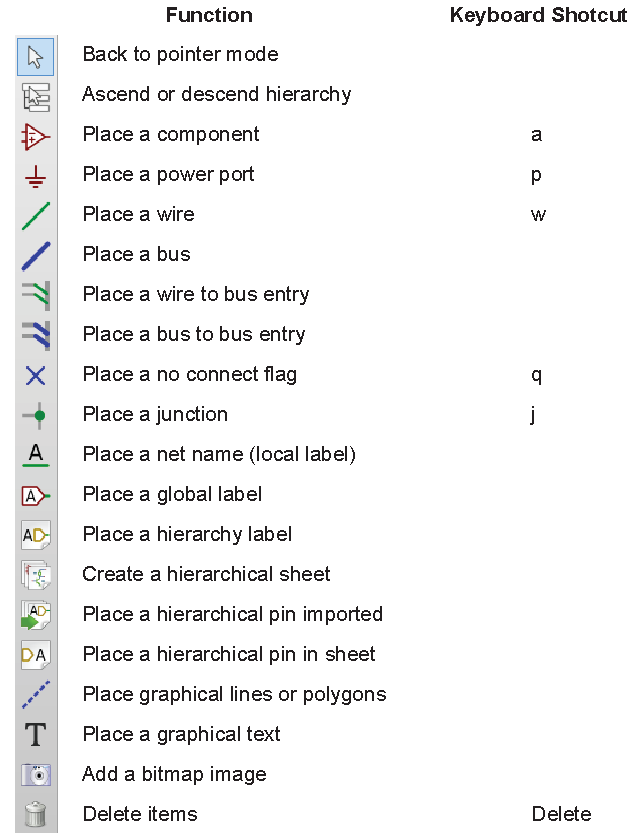
\includegraphics{eeschema-toolbar}
					\caption{Eeschema toolbar icons.}
					\label{fig:eeschema-toolbar}
				\end{figure}
				
			\item Click anywhere on the schematic, a dialog box should appear. 
				\begin{figure}[h]
					\centering
					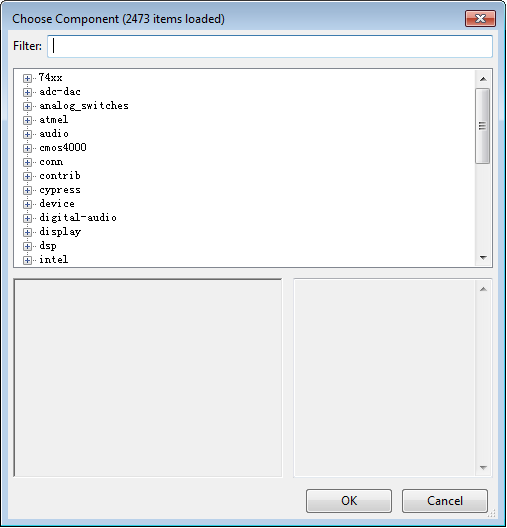
\includegraphics[width=3in]{place-component.png}
					\caption{Place component dialog box.}
					\label{fig:place-component}
				\end{figure}

			\item We’ll add our first item, the ATmega328P microcontroller, from the ``atmel'' library. Select the ``atmel'' entry, and click ``OK''. A new dialog box appears for you select the particular device, the “ATMEGA328P-P”. Click ``OK''. Note that if you already know the name of the component, you can simply start typing the name and Eeschema will filter out the components with the same initial characters. It wouldn't take long before you arrive at your desired component.
			
			\item The ATmega328P symbol should now cling to your mouse cursor. Click on the schematic to place it at a location you like. 
			\item A number of component editing operations are available by right clicking on the component. Some of the operations have keyboard shortcut. The general way to use the shortcut is to place the cursor on the component and press the corresponding shortcut key. Pressing the ``ESC'' key will cancel the current operation. 
			
			\begin{figure}[h]
				\centering
				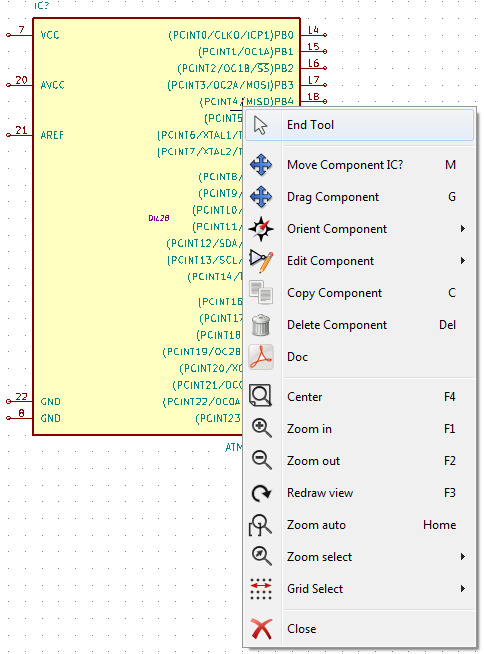
\includegraphics[width=3in]{edit-component}
				\caption{Edit component pop-up menu.}
				\label{fig:edit-component}
			\end{figure}

				\begin{enumerate}
					\item ``Move component'' will move the component and break all circuit connections to it. To retain the connections, use ``Drag component''. 
					\item ``Orient component'' has further options to rotate and mirror the component. Experiment the shortcuts by pressing ``r'' or ``y'' while placing the cursor on the component.
					\item ``Edit component$\rightarrow$ Edit'' will bring up a dialog box that allows you to edit all of the component properties. 
						\begin{enumerate}
							\item The ``Reference'' and ``Value'' are the two properties that you are most likely to edit in this dialog box. ``Reference'' is the annotation of the component. In this case, it should read ``IC1''. You may also write it as ``IC?'' where the ``?'' is a placeholder for a numeric value. KiCad can auto annotate the components and assign a unique value for each component. 
							\item The \emph{Value} entry is usually used to mark the component value. For resistors, capacitors, and inductors for examples, the \emph{Value} can simply be their corresponding resistance, capacitance, and inductance values. For this ATmega microcontroller we will simply use the \emph{Value} to mark the component’s name. 
						\end{enumerate}
				\end{enumerate}
		\end{enumerate}
	\item Follow a similar procedure to place the other circuit components. The following table lists which library they belong to. Arrange the components to make connecting them easier. 
		\begin{enumerate}
			\item Note that the Vcc and ground symbols, and all other symbols related to providing power to the circuits, are organized into the \emph{power} library. They can be accessed directly by clicking the \emph{Place a power port} button from the toolbar on the right. Place a \emph{Vcc} and several \emph{GND} pins where necessary.
		\end{enumerate}
	\item Connect the components together according to Fix. xxx by placing wires between corresponding pins. To start placing a wire, click on the ``Place a wire'' button, then click on the starting point, and finish by clicking on the endpoint of the wire. It is often easier to use the keyboard shortcut. First move your cursor to the starting point and then press the ``w'' key. A wire is started at the cursor location. Click at the endpoint to finish the connection. 
	
	\item The schematic drawing can become hard to read if there are too many wire crossovers. Named netlist can be used to alleviate the issue. Although our example circuit is quite simple and easy to read, we will still use it to illustrate how to “clean up” the schematic with named net.
		\begin{enumerate}
			\item Delete the wire between the ATmega328P’s PB1 pin and the 7-segment LED’s DP pin.
			\item Draw a short section of wire on the ATmega328P’s PB1 pin; one of the ends of the wire is now floating. 
			\item Click the ``Place a net name (local label)'' button and then click on the schematic. A dialog box will appear, input ``DP'' in the ``Text'' field, and click ``OK''. The text ``DP'' can now be seen to cling on the cursor. 
			\item Click on the floating terminal of the short wire on the PB1 pin to finish naming a net. You should now see the text DP attached to the wire on the ``PB1'' pin; the bubble at the floating end of the wire has also disappeared. 
			\item Repeat step b--d for the DP pin of the 7-segment LED. 
			The ATmega328P’s PB1 pin and the 7-segment LED’s DP pin are now connected by the net name ``DP'' even though there is no direct wire connection on the schematic view. 
			\item Repeat the step a--e for the connection between ATmega328P’s PB4 pin and the push button. The schematic should now look like the following.  
		\end{enumerate}
	
	\item In most circuits, the unused pins can be left floating. In this example, however, we will terminate all the unused pins by placing a no connect label on them; this tells KiCad to ignore these pins during the electrical rule check (ERC).
	
	\item The schematic capture is now almost done. Notice that the references to some of the components still have question marks. For example, the two capacitors connected to the crystal oscillator look identical to each other; we need to differentiate them. In KiCad, we do this by annotating the schematic, i.e. giving each component a unique identifier (reference). Annotation can be done manually by changing the ``Reference'' property of a component and making sure that each reference is unique, but it is much easier to let KiCad do the annotation automatically. 
		\begin{enumerate}
			\item Click the ``Annotate'' button. 
			\item A dialog box appears. The options are all self-explanatory. 
			\item Click the ``Annotation'' button to finish. You must have noticed that you can ``un-annotate'' the schematic by clicking the ``Clear annotation'' button. 
			\item After annotation, you should see that all the components are numbered. 
		\end{enumerate}
	\item It is always a good idea to run an ERC before proceeding. ERC checks the electrical connections between components and try to detect potential errors in the schematic.
	
	\item Once you’ve passed the ERC, generate a netlist by clicking the ``Generate netlist'' button.
	
	\item This will create a netlist file that describes the circuit connections. The netlist file will be used to guide the PCB layout process.
	
	\item The final schematic should look like the following.
\end{enumerate}

\subsection{Creating or Editing Schematic Symbols}
Sometimes you run into a situation where you can’t find a proper symbol in the default KiCad library for the component that you want to use. The following steps will show you how to create a schematic symbol of your own. 

\begin{enumerate}
	\item From the Eeschema window, click the “Library editor” button .
	The library editor window should appear.
	\item Click the “Select working library” button  to set the current working library. A dialog box should appear. 
	
	
\end{enumerate}
\subsection{PCB Layout}
\subsection{Associating schematic symbols with footprint}
\subsection{Creating or Editing Footprint}
\subsection{Generate Fabrication Files}

\section{Advanced Topics}

\subsection{Controlled Impedance Lines}

* Transmission line parameter calculator: http://wcalc.sourceforge.net/

\newpage

\bibliography{pcb}
\bibliographystyle{plain}

\end{document}
